\documentclass[11pt]{article}

\usepackage[margin=1in]{geometry}
\usepackage{fontspec}
\usepackage{setspace}
\usepackage{booktabs}
\usepackage{array}
\usepackage{graphicx}
\usepackage{hyperref}
\usepackage{tikz}
\usetikzlibrary{arrows.meta,positioning,shapes.geometric}

\IfFontExistsTF{Times New Roman}
  {\setmainfont{Times New Roman}}
  {\setmainfont{TeX Gyre Termes}}

\onehalfspacing
\setlength{\parindent}{0pt}
\setlength{\parskip}{0.45em}
\setlength{\emergencystretch}{2em}

\hypersetup{
  colorlinks=true,
  linkcolor=black,
  urlcolor=black,
  citecolor=black
}

\newcommand{\projecttitle}{Design and Pilot Evaluation of a Portable Benchmarking Methodology for Memory-Bound Parallel Workloads on ARM64 and x86-64 Systems}

\begin{document}

\begin{titlepage}
\centering
\vspace*{1.0in}
{\Large \textbf{Interim Project Report}\par}
\vspace{0.5in}
{\large \textbf{\projecttitle}\par}
\vspace{0.8in}
{\large Rufat Guliyev\par}
\vspace{0.25in}
{\large George Washington University\par}
\vspace{0.25in}
{\large CSCI 6918: Guided Research for Graduate Students II\par}
\vfill
{\large July 14, 2026\par}
\end{titlepage}

\section{Introduction}

The goal of this guided research project is to develop and pilot a portable methodology for evaluating memory-bound parallel workloads on ARM64 and x86-64 systems. The project is intentionally not a general CPU-performance comparison. Instead, it focuses on low-arithmetic-intensity kernels whose execution time is dominated by data movement through cache and main memory. This framing matters because many scientific and data-processing kernels do not primarily stress peak floating-point throughput; they stress cache locality, memory bandwidth, working-set size, prefetching behavior, and the ability of additional threads to use shared memory bandwidth effectively.

The central research question for the project is how a portable benchmark and analysis workflow can be designed and validated using accessible consumer hardware. The two pilot systems are an Apple M4 MacBook Air, representing an accessible ARM64 platform, and a desktop PC with an Intel Core i5-12400F, representing an accessible x86-64 platform. These machines are not controlled equivalents. They differ in processor design, memory subsystem, operating system, power behavior, cooling, compiler environment, and OpenMP runtime details. Therefore, the current results should be read as methodology validation and workload-specific pilot evidence, not as a universal claim about ARM64 or x86-64 superiority.

At the interim stage, the project has progressed beyond the minimum milestone described in the proposal. The original interim target was a focused literature review, an initial benchmark design, an initial implementation, preliminary results from at least one machine, initial plots, and an updated risk assessment. The current state includes a working benchmark suite, integration of official STREAM as an established baseline, custom memory-bound kernels, OpenMP builds on both pilot machines, metadata collection, reproducible experiment scripts, CSV output, automated summaries, plot generation, and full pilot sweeps on both systems.

\section{Technical Approach}

The technical approach is to build a reproducible measurement pipeline around memory-bound kernels rather than around isolated benchmark runs. Each benchmark is compiled with a documented compiler, executed through a repeatable driver, written to a normalized CSV schema, summarized statistically, and analyzed with conservative interpretation. The pipeline combines established benchmarks where they are useful with custom kernels where the project needs controlled access patterns or a common output format.

STREAM is used as the recognized baseline for sustainable memory bandwidth behavior. Its Copy, Scale, Add, and Triad kernels are valuable because they are widely understood and provide a reference point for memory throughput. The project does not attempt to replace STREAM. Instead, it wraps and normalizes STREAM output so that it can be compared with the custom measurement pipeline. The custom benchmark executable currently includes Copy, Scale, Add, Triad, sequential traversal, strided traversal, vector reduction, and a one-dimensional stencil. These kernels cover contiguous streaming, reuse, reductions, and access patterns with reduced spatial locality.

The workflow records runtime, effective bandwidth, speedup, scaling efficiency, checksum values, compiler information, warm-up count, timed iteration count, and machine identifier. Experiments are repeated multiple times, and analysis uses medians across repetitions. Coefficient of variation is used to identify unstable groups. For the full pilot sweep, each machine produced 1,372 result rows, representing 196 matched workload groups when grouped by kernel, element count, stride, and thread count.

Several decisions changed from the original proposal as implementation progressed. First, the project now treats official STREAM as a first-class established benchmark instead of relying only on custom STREAM-style kernels. Second, the measurement design was revised to batch multiple kernel iterations inside each timed repetition, because early timing runs showed that small or sparse-stride cases could produce regions that were too short to be stable. Third, strided traversal was corrected to use an OpenMP reduction so that multi-thread results measure actual parallel work rather than a serial loop under a multi-thread configuration. Fourth, the experiment runner now uses a shared configuration for both machines, which improves comparability at the pipeline level.

The main technologies are C, OpenMP, LLVM/Clang, Python, CSV files, and LaTeX. On macOS, Homebrew LLVM/Clang and \texttt{libomp} are used because Apple Clang does not provide the needed OpenMP support by default. On the Intel desktop, Clang 22.1.8 links against \texttt{libomp.so}. Python scripts drive experiments, normalize outputs, collect metadata, summarize results, compare machines, and generate plots. The report itself is compiled with Tectonic.

\section{Software Architecture}

Figure~\ref{fig:architecture} summarizes the current software architecture. The design separates benchmark execution from analysis. This separation is important because the same raw measurement pipeline can be reused when additional machines or kernels are added.

\begin{figure}[htbp]
\centering
\resizebox{\textwidth}{!}{%
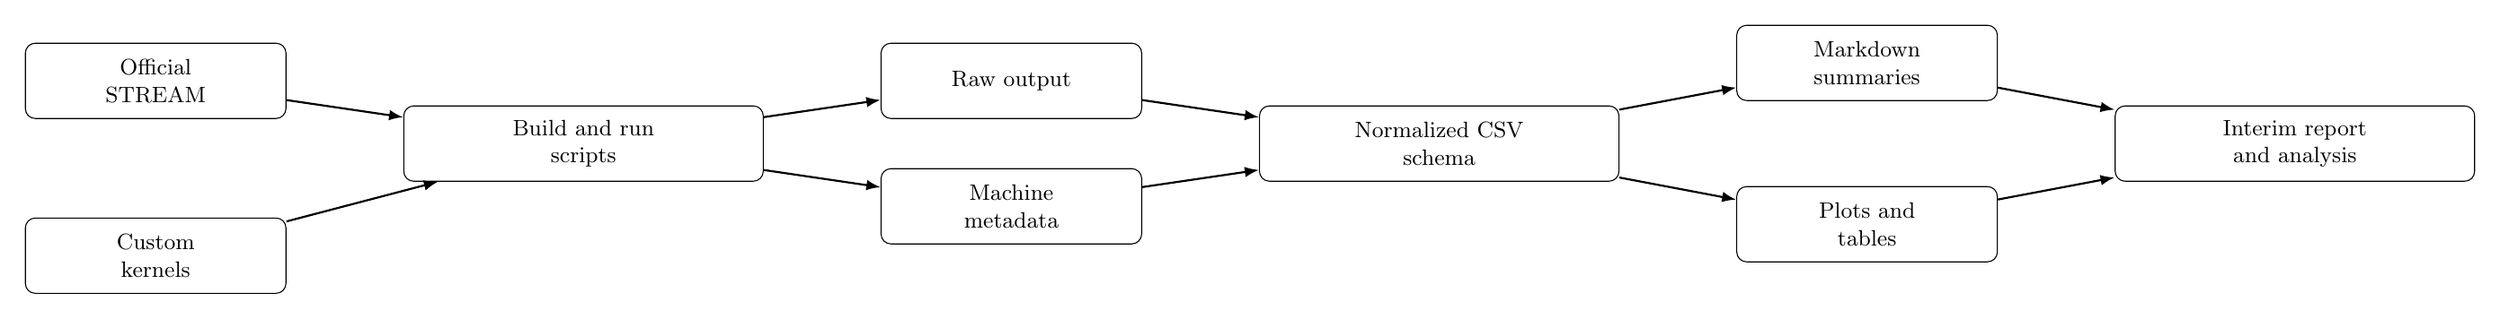
\begin{tikzpicture}[
  node distance=0.55in and 0.65in,
  box/.style={draw, rounded corners, align=center, minimum width=1.45in, minimum height=0.42in, font=\small},
  wide/.style={draw, rounded corners, align=center, minimum width=2.0in, minimum height=0.42in, font=\small},
  arrow/.style={-{Latex[length=2mm]}, thick}
]
\node[box] (stream) {Official\\STREAM};
\node[box, below=of stream] (custom) {Custom\\kernels};
\node[wide, right=of stream, yshift=-0.35in] (runner) {Build and run\\scripts};
\node[box, right=of runner, yshift=0.35in] (raw) {Raw output};
\node[box, right=of runner, yshift=-0.35in] (metadata) {Machine\\metadata};
\node[wide, right=of raw, yshift=-0.35in] (csv) {Normalized CSV\\schema};
\node[box, right=of csv, yshift=0.45in] (summary) {Markdown\\summaries};
\node[box, right=of csv, yshift=-0.45in] (plots) {Plots and\\tables};
\node[wide, right=of summary, yshift=-0.45in] (report) {Interim report\\and analysis};

\draw[arrow] (stream) -- (runner);
\draw[arrow] (custom) -- (runner);
\draw[arrow] (runner) -- (raw);
\draw[arrow] (runner) -- (metadata);
\draw[arrow] (raw) -- (csv);
\draw[arrow] (metadata) -- (csv);
\draw[arrow] (csv) -- (summary);
\draw[arrow] (csv) -- (plots);
\draw[arrow] (summary) -- (report);
\draw[arrow] (plots) -- (report);
\end{tikzpicture}
}
\caption{Software architecture and data flow for the memory-bound benchmark pipeline.}
\label{fig:architecture}
\end{figure}

The benchmark sources are organized into external and custom components. The external component contains official STREAM source files and wrapper scripts. The custom component contains the project's C kernels and shared utilities. A Makefile builds the benchmark executable with either serial or OpenMP support, and the experiment scripts choose machine identifiers, thread counts, working-set sizes, strides, repetitions, warm-ups, and timed iteration counts.

Data flow begins with a configured run. The runner invokes the benchmark executable or STREAM wrapper, records raw output where appropriate, and writes normalized CSV rows. Metadata collection records the machine model, operating system, compiler, OpenMP runtime, memory size, and other fields that support interpretation. Analysis scripts then compute medians, speedups, efficiencies, and coefficients of variation. A cross-machine comparison script matches results by kernel, element count, stride, and thread count, ensuring that comparisons are made only between equivalent workload groups.

\section{Experimental Data}

The project does not use an external application data set. The data set for this interim report is the experimental measurement data produced by the benchmark pipeline. This is appropriate for the project because the research object is a measurement methodology for memory-bound workloads. The important data are the structured observations generated by controlled kernels across working-set sizes and thread counts.

The current full pilot data set contains one Mac sweep and one Intel sweep. Each sweep contains 1,372 result rows. The two sweeps match exactly at the workload-group level, producing 196 matched groups and no unmatched groups. Each row records the source benchmark, machine identifier, kernel, element count, useful byte count, stride, thread count, repetition, warm-up count, timed iteration count, runtime, effective bandwidth, checksum, compiler, and compiler flags.

\begin{table}[htbp]
\caption{Pilot systems used for the interim measurements.}
\label{tab:systems}
\centering
\small
\begin{tabular}{p{1.35in}p{2.05in}p{2.25in}}
\toprule
System & Hardware and OS & Compiler and OpenMP runtime \\
\midrule
Mac pilot system & Apple M4 MacBook Air, 10 cores, 16 GB memory, macOS 26.5.2 & Homebrew Clang 22.1.8 with Homebrew \texttt{libomp}; Apple Clang recorded but not used for OpenMP runs \\
Intel pilot system & Intel Core i5-12400F desktop, 6 cores, 15.45 GiB memory, CachyOS Linux & Clang 22.1.8 with \texttt{libomp.so} \\
\bottomrule
\end{tabular}
\end{table}

Table~\ref{tab:large-summary} shows selected large working-set results from the cross-machine pilot comparison. The table is included to demonstrate the type of analysis the pipeline now supports. It should not be read as a final architecture ranking, because the machines are not controlled equivalents.

\begin{table}[htbp]
\caption{Selected 256 MiB working-set results from the matched pilot sweeps.}
\label{tab:large-summary}
\centering
\small
\begin{tabular}{lrrrr}
\toprule
Workload & Threads & Mac M4 GB/s & Intel i5 GB/s & Mac/Intel \\
\midrule
Sequential traversal & 1 & 15.14 & 15.98 & 0.95 \\
Reduction & 1 & 14.89 & 15.04 & 0.99 \\
Reduction & 4 & 56.14 & 44.94 & 1.25 \\
Triad & 1 & 92.54 & 29.11 & 3.18 \\
Triad & 2 & 94.35 & 32.04 & 2.94 \\
Triad & 4 & 94.09 & 42.54 & 2.21 \\
Stencil1D & 1 & 167.13 & 47.56 & 3.51 \\
Stencil1D & 4 & 195.83 & 73.68 & 2.66 \\
\bottomrule
\end{tabular}
\end{table}

Figure~\ref{fig:triad-bars} shows large Triad bandwidth by thread count. The Mac M4 result is already near saturation at one thread for this workload, while the Intel desktop continues to improve from one to four threads. This is a memory-system observation about this workload and these systems, not a general statement about processor quality.

\begin{figure}[htbp]
\centering
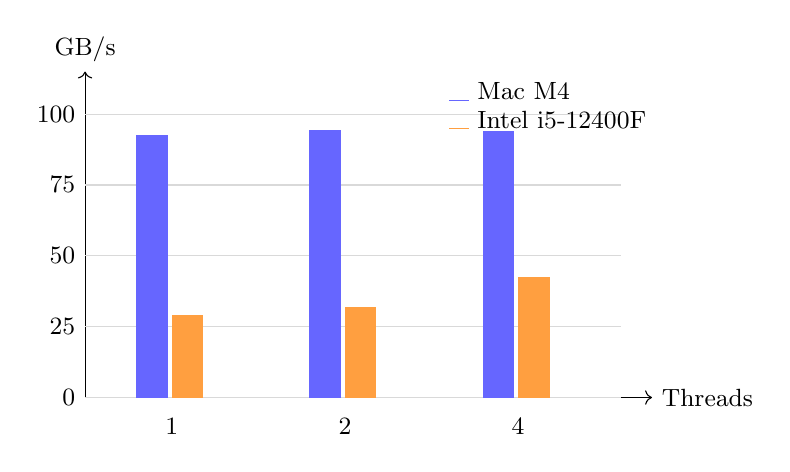
\begin{tikzpicture}[x=1cm,y=0.036cm]
  \draw[->] (0,0) -- (7.2,0) node[right] {\small Threads};
  \draw[->] (0,0) -- (0,115) node[above] {\small GB/s};
  \foreach \y in {0,25,50,75,100} {
    \draw[gray!30] (0,\y) -- (6.8,\y);
    \node[left] at (0,\y) {\small \y};
  }
  \foreach \x/\label in {1.1/1,3.3/2,5.5/4} {
    \node[below] at (\x,-4) {\small \label};
  }
  \fill[blue!60] (0.65,0) rectangle (1.05,92.54);
  \fill[orange!75] (1.10,0) rectangle (1.50,29.11);
  \fill[blue!60] (2.85,0) rectangle (3.25,94.35);
  \fill[orange!75] (3.30,0) rectangle (3.70,32.04);
  \fill[blue!60] (5.05,0) rectangle (5.45,94.09);
  \fill[orange!75] (5.50,0) rectangle (5.90,42.54);
  \node[anchor=west] at (4.5,108) {\small \tikz\fill[blue!60] (0,0) rectangle (0.25,0.12); Mac M4};
  \node[anchor=west] at (4.5,98) {\small \tikz\fill[orange!75] (0,0) rectangle (0.25,0.12); Intel i5-12400F};
\end{tikzpicture}
\caption{Large working-set Triad effective bandwidth at 256 MiB.}
\label{fig:triad-bars}
\end{figure}

Figure~\ref{fig:stride-line} shows the effect of stride on useful bandwidth at the 256 MiB working-set size with one thread. Both systems lose useful bandwidth as stride increases. This is consistent with reduced spatial locality and cache-line underutilization. The reported bandwidth is useful payload bandwidth, not a direct count of all physical cache-line traffic.

\begin{figure}[htbp]
\centering
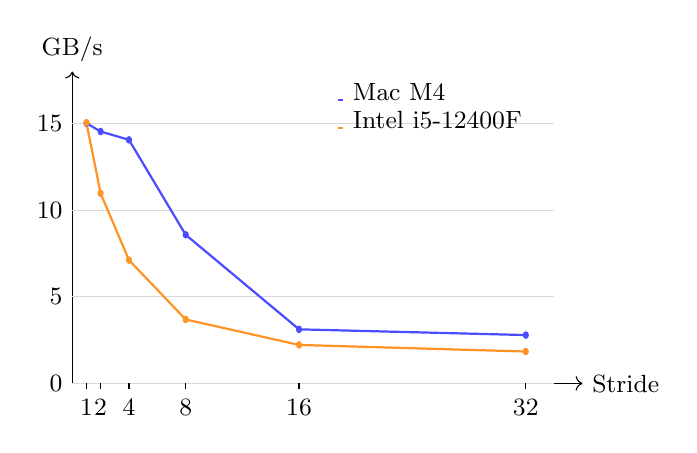
\begin{tikzpicture}[x=0.18cm,y=0.22cm]
  \draw[->] (0,0) -- (36,0) node[right] {\small Stride};
  \draw[->] (0,0) -- (0,18) node[above] {\small GB/s};
  \foreach \y in {0,5,10,15} {
    \draw[gray!30] (0,\y) -- (34,\y);
    \node[left] at (0,\y) {\small \y};
  }
  \foreach \x in {1,2,4,8,16,32} {
    \draw (\x,0) -- (\x,-0.35);
    \node[below] at (\x,-0.35) {\small \x};
  }
  \draw[blue!70, thick] plot coordinates {(1,15.02) (2,14.54) (4,14.06) (8,8.58) (16,3.12) (32,2.79)};
  \draw[orange!85, thick] plot coordinates {(1,15.05) (2,10.97) (4,7.12) (8,3.69) (16,2.22) (32,1.84)};
  \foreach \x/\y in {1/15.02,2/14.54,4/14.06,8/8.58,16/3.12,32/2.79} {
    \fill[blue!70] (\x,\y) circle (0.22);
  }
  \foreach \x/\y in {1/15.05,2/10.97,4/7.12,8/3.69,16/2.22,32/1.84} {
    \fill[orange!85] (\x,\y) circle (0.22);
  }
  \node[anchor=west] at (18,16.8) {\small \tikz\draw[blue!70, thick] (0,0) -- (0.35,0); Mac M4};
  \node[anchor=west] at (18,15.2) {\small \tikz\draw[orange!85, thick] (0,0) -- (0.35,0); Intel i5-12400F};
\end{tikzpicture}
\caption{Useful bandwidth for one-thread strided traversal at 256 MiB.}
\label{fig:stride-line}
\end{figure}

\section{Coding and Testing Completed}

The implementation work to date covers the full pipeline from source code to analysis artifacts. The benchmark suite structure separates custom source code, external benchmark integration, configuration files, scripts, results, plots, and documentation. The custom benchmark executable supports serial and OpenMP builds. It validates requested thread counts, disables dynamic OpenMP teams, performs warm-up calls, executes batched timed iterations, computes checksums outside the timed region, and writes normalized CSV rows.

The official STREAM integration has also been completed. Official STREAM source files were downloaded from the University of Virginia STREAM source directory and placed under the external benchmark area. A wrapper builds STREAM with LLVM/Clang and OpenMP, runs selected thread counts, saves raw output, and normalizes Copy, Scale, Add, and Triad rows into the project CSV schema. A comparison helper checks whether custom STREAM-style kernels and official STREAM show compatible bandwidth trends. This strengthens the methodology because it shows that the project can integrate established benchmarks rather than relying only on original code.

Testing has been iterative. Early serial smoke tests verified that the custom executable could compile and emit CSV rows. OpenMP smoke tests then verified that Homebrew LLVM on the Mac and LLVM/Clang on the Intel desktop could compile and run multi-threaded kernels. Initial validation exposed strict C portability issues on Linux, including missing feature-test macros for \texttt{posix\_memalign} and \texttt{clock\_gettime}; these were fixed. The one-dimensional stencil loop was also revised to satisfy OpenMP canonical loop requirements.

The most important testing revision was the second-stage measurement correction. Early short runs showed that some timings were too brief, especially for cache-resident or sparse-stride cases. The runner was extended to support multiple timed iterations per repetition, and strided workloads now scale timed iterations by stride so that useful-access counts remain more comparable. After this correction, the Mac full sweep reduced groups above the 10 percent coefficient-of-variation threshold from 30 to 11. The Intel full sweep reported zero groups above that threshold.

\section{Revisions to Deliverables}

The core deliverable remains the same as in the proposal: a reusable memory-bound benchmark and analysis workflow. However, the implementation has become more mature and more concrete than originally expected for the interim stage. The proposal described initial implementation and preliminary results from at least one machine as the interim target. The current deliverable already includes two-machine pilot results, official STREAM integration, custom kernels, metadata capture, machine comparison, summaries, and plots.

The deliverables have also shifted slightly away from adding more kernels and toward improving measurement quality. Optional kernels such as a two-dimensional stencil or matrix-vector multiplication are not being prioritized at this stage. That is a deliberate scope decision. The existing kernels already cover contiguous streaming, strided access, reductions, and stencil-style reuse. The higher-value work for the remainder of the course is to strengthen reproducibility, clean up documentation, refine interpretation, and prepare a final demonstration that shows the full workflow.

Another revision is that compiler consistency has become a formal part of the deliverable. The project now standardizes on LLVM/Clang where possible. GCC remains a fallback, but the current Mac and Intel pilot results both use Clang 22.1.8 for OpenMP execution, which reduces one source of toolchain variation.

\section{Risks}

The main scientific risk remains hardware inequality. The Apple M4 MacBook Air and Intel Core i5-12400F desktop are useful pilot platforms, but they are not controlled equivalents. The report therefore avoids broad architecture claims. It reports workload-specific behavior, records machine metadata, and treats the local comparison as validation of a portable methodology.

Measurement noise is another important risk. Laptop thermals, background processes, power management, OS scheduler behavior, and OpenMP thread placement can affect results. This risk is visible in the Mac full sweep, where 11 of 196 groups exceeded the 10 percent coefficient-of-variation threshold. Most of those warnings occur in four-thread stencil or strided cases. The Intel sweep was more stable, with zero groups above the threshold. The mitigation is to report medians, track coefficient of variation, avoid hiding unstable groups, and document macOS affinity limitations.

OpenMP portability remains a practical risk. The Mac requires Homebrew LLVM/Clang and \texttt{libomp}; Apple Clang alone is insufficient for the intended OpenMP experiments. The Intel system uses Clang and \texttt{libomp.so}. This risk has been mitigated for the current pilot machines, but future machines will still require explicit compiler and runtime documentation.

Finally, there is a scope risk. The project could expand into many additional benchmarks, performance counters, or machine-specific tuning steps. For the interim stage, the best mitigation is to freeze the current pilot data set and focus on reporting the pipeline clearly. Further extensions should be added only after the current workflow is documented and reproducible.

\section{Assessment of Status}

The project is ahead of the original interim expectation. The core benchmark-and-analysis pipeline exists and has been exercised on both target systems. The current implementation can build, run, collect metadata, produce structured CSV output, summarize variation and speedup, generate plots, and compare matched workload groups across machines. The current results also demonstrate the intended memory-bound framing: Triad shows bandwidth saturation behavior, strided traversal shows reduced useful bandwidth as locality worsens, and repeated trials provide a basis for judging measurement stability.

The remaining work is mostly about consolidation rather than rescue. The final report should refine the analysis, select a compact figure set, improve reproducibility documentation, and clearly separate methodology validation from hardware conclusions. The final demonstration should show the workflow end to end: compiling, running a small experiment, generating CSV output, producing a summary or plot, and explaining how the same process scales to the full pilot data set.

The most important discipline for the next phase is to avoid unnecessary scope expansion. Adding more kernels or tools would be useful only if they answer a clearly missing question. At this stage, the project already has enough experimental evidence to support the course objective. The stronger contribution is to make the methodology coherent, reproducible, and honestly interpreted.

\end{document}
